\documentclass[a4paper,12pt,oneside]{book}
\usepackage[utf8]{inputenc}
\title{}
\author{Rachel Morris}
\date{\today}

\usepackage{rachwidgets}
\usepackage{fancyhdr}
\usepackage{lastpage}
\usepackage{boxedminipage}
\usepackage{fancyvrb}
\usepackage{xcolor}

\newcommand{\laClass}{CS 250\ }
\newcommand{\laSemester}{Fall 2017\ }
\newcommand{\laLab}{Lab 17: GitHub\ }
\newcounter{question}

\pagestyle{fancy}
\fancyhf{}
\lhead{\laClass}
\chead{\laSemester}
\rhead{\laLab}
\rfoot{\thepage\ of \pageref{LastPage}}
\lfoot{By Rachel Morris, \footnotesize last updated \today}

\renewcommand{\headrulewidth}{2pt}
\renewcommand{\footrulewidth}{1pt}


\begin{document}

    \chapter*{\laLab} \stepcounter{chapter}

        \section{Information}
            \paragraph{ Topics: } Debugger
            \paragraph{ Turn in: } asdf


        \begin{center}
            
\includegraphics[width=10cm]{images/octocat.png}
        \end{center}

        \tableofcontents
            
% ----------------------------------------------------------------------
% ----------------------------------------------------------------------
% ----------------------------------------------------------------------

    \newpage

    \section{About Source Control, Git, and GitHub}

    \paragraph{What is Source Control?}

        Source Control (aka Version Control or Revision Control) is a
        type of software system that allows people to keep track of their
        changes over time, back up their work to a server, and make
        merging code between different people (or different machines)
        easier.

        \subparagraph{Storing your work on a server}
            By storing your work on a server on the internet, you can access
            your work from anywhere, simply by using a command like ``clone''
            to pull down all the changes. No need to carry around a flash drive!

            If you store your work on a source hosting service like BitBucket
            or GitHub, then you can also view your work through their web-based
            interface as-needed.

            \begin{figure}[h]
                \centering
                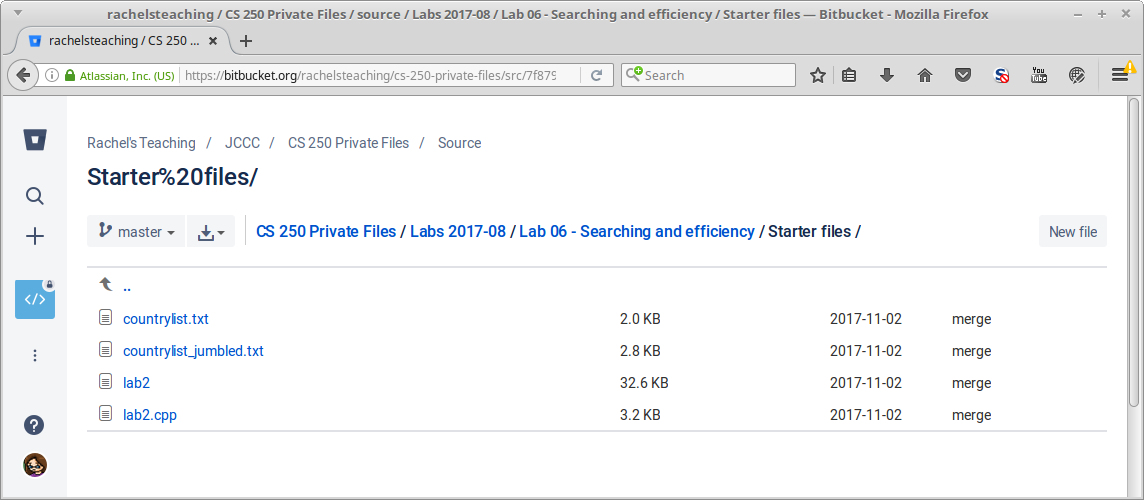
\includegraphics[width=12cm]{images/bitbucket-view.png}
                \caption{Viewing a list of files on BitBucket}
            \end{figure}

            \begin{figure}[h]
                \centering
                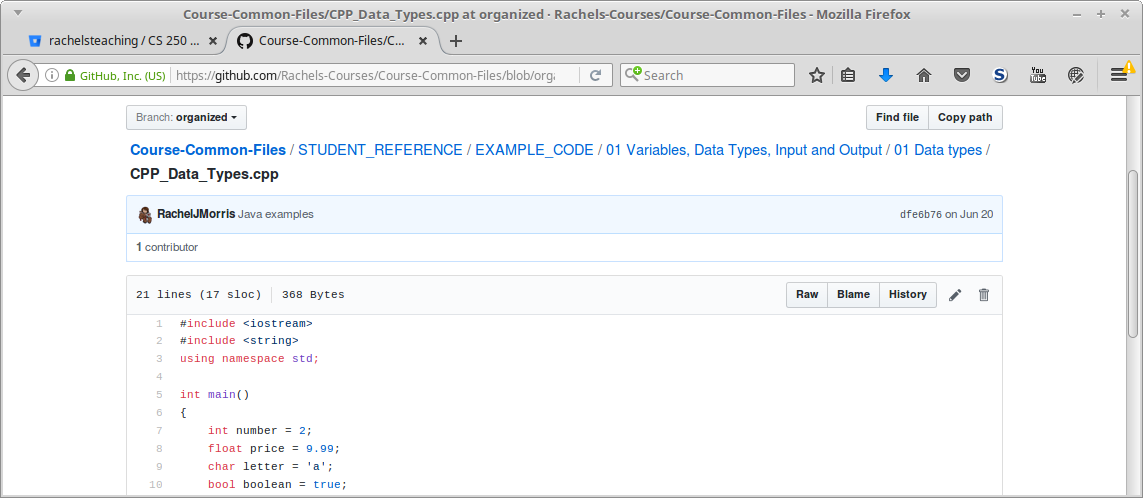
\includegraphics[width=12cm]{images/github-view.png}
                \caption{Viewing source code on GitHub}
            \end{figure}

        \newpage

        \subparagraph{Keeping track of changes}
            Each source control solution also has features to let you
            review the changes to your code over time. By associating
            your changes with a ``commit'' and a ``commit message'',
            you can effectively make snapshots of your code over time.

            \begin{figure}[h]
                \centering
                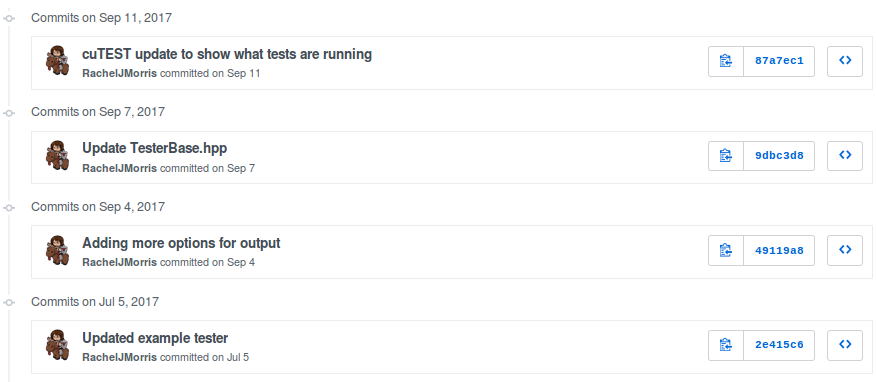
\includegraphics[width=14cm]{images/github-history.png}
                \caption{Viewing change history on GitHub}
            \end{figure}

            And, besides just viewing a list of changes, you can also
            do a ``diff'' to see exactly what changed between commits,
            line-by-line.

            \begin{figure}[h]
                \centering
                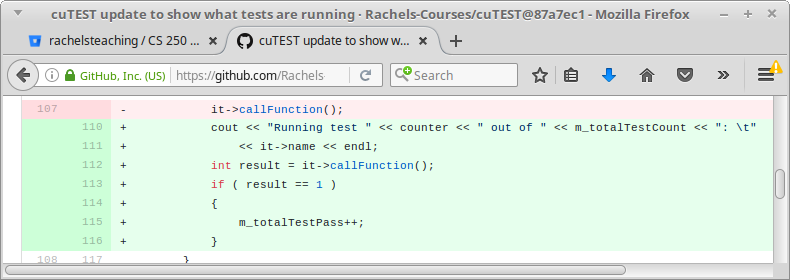
\includegraphics[width=14cm]{images/git-diff.png}
                \caption{Viewing line changes in GitHub - Red for lines removed, green for lines added}
            \end{figure}

        \subparagraph{Merging}
            If you're working across multiple computers, or working with other people,
            you may have different versions of the code on different machines.
            With a source control program, it will take care of merging
            in different changes to the same file - and if it can't figure out
            how to automatically merge files, it will give you some interface
            to do it manually in an easier manner.

            \begin{figure}[h]
                \centering
                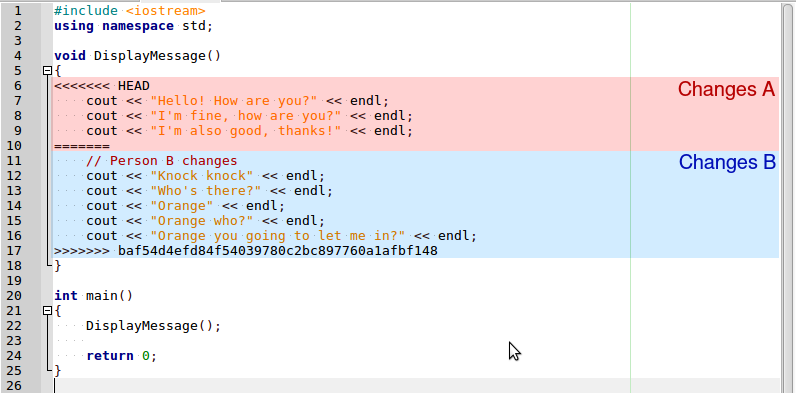
\includegraphics[width=14cm]{images/merge-conflict-b.png}
                \caption{Merge conflict flags added to the code by Git}
            \end{figure}

            In the case above, two people edited the same code around
            the same time. Once Person A pulled the latest code from the
            server, the knock knock joke was already committed and pushed up.
            Git pulled the latest code and tried to merge, but couldn't figure
            out which was the correct version for this function, so instead
            it added markers around the part it didn't know how to merge
            on its own. That way, the programer can manually decide what
            to save and what to remove.

    \hrulefill

    \paragraph{What are some version control systems?}

        Some common version control systems are:

        \subparagraph{Git} ~\\

            Git is a popular source control system for open source projects
            and work that doesn't use Microsoft products (usually, Microsoft
            shops use TFS). Git was created by the maker of Linux, Linus Torvalds,
            and it is open source.

            ~\\
            https://git-scm.com/

        \newpage

        \subparagraph{Mercurial} ~\\

            Mercurial is another popular source control system, built
            by Atlassian (who also make Jira and BitBucket).
            Mercurial is available as Free software under GNU GPL v2.

            ~\\
            https://www.mercurial-scm.org/

        \subparagraph{TFS} ~\\

            Team Foundation Server (TFS) is Microsoft's source control
            solution, which is commonly used at companies that use
            Microsoft tech, such as C\#, ASP.NET, and others.

            ~\\
            https://www.visualstudio.com/tfs/

        \subparagraph{Subversion (SVN)} ~\\

            Subversion is an older source control solution, and (in my opinion)
            it is less robust than the above three. However, it is still
            used in various places, so you might run into it sooner or later.
            
            ~\\
            https://subversion.apache.org/

    \newpage

    \paragraph{What are some source hosting sites?}

        You can always host your own source control server on your local
        machine or on a server you run, but you can also host your code
        on a hosting service.

        Many hosting services allow free hosting for public repositories,
        so they are open source-friendly. Otherwise, they may charge
        for private repositories, such as for hosting a business' product
        repositories. It depends on the service!

        \subparagraph{GitHub}

            GitHub allows you to host Git projects. It is free if your
            repository is public, but costs if you have private repositories.

        \subparagraph{Bitbucket}

            Bitbucket can host Mercurial and Git projects. It is free
            for public and private repositories. Private is free for
            small teams of up to 5 users. Bitbucket is ran by the
            creators of Mercurial, Atlassian.

            (Usually I host my open source stuff on GitHub and my
            startup's private repos here.)

        \subparagraph{CodePlex}

            CodePlex is Microsoft's hosting solution for open source projects.
            It supports Mercurial, TFS, SVN, and Git.

        \subparagraph{Sourceforge}

            Sourceforge is a popular hosting site for open source projects.
            It supports SVN, Git, Mercurial, and some other source control systems.

    \hrulefill

    \paragraph{What are we doing?}

        For this lab, you will be creating a GitHub account and using Git
        to upload your programs from this semester to a CS 250 repository.
        This way, it will be available for you to reference in the future
        as needed, but also will be visible to potential employers.
        It is good to keep a portfolio of your work on GitHub so that
        potential employers can see what you've worked on. Your code doesn't
        have to be perfect or beautiful, but it is good to see what you've
        accomplished.

    \hrulefill

    \section{Getting started}

        \subsection{Creating a GitHub account}

            First, create a GitHub account at https://github.com/ .
            You will need to specify an email address, username, and password.
            You can use your school email or your person email - whichever
            you're less likely to forget. :)

            When it asks what plan you'd like, select the free once.

            Once you're finished, you will have a profile at
            github.com/YOUR-NAME You will be able to create repositories
            from this directory.

        \subsection{Creating a CS 250 repository}

            From the web interface, you will create a repository for
            the CS 250 class.

            \paragraph{What is a repository?}

                You will generally create one repository per project
                that you're working on. For example, id software has
                the following repositories...

                \begin{itemize}
                    \item   Quake III Arena \\ https://github.com/id-Software/Quake-III-Arena
                    \item   DOOM 3 \\ https://github.com/id-Software/DOOM-3
                    \item   Wolfenstein 3D \\ https://github.com/id-Software/wolf3d
                \end{itemize}

                So essentially, each game has its own repository.

                In this lab's case, you will throw all your CS 250 projects
                into one repository, but for future projects, you could
                put each project in its own repository.

            \paragraph{Creating a repository}

                From your GitHub profile page, github.com/YOUR-NAME,
                click on the \textbf{Repositories} tab, then click the
                \textbf{New} button.

                \begin{figure}[h]
                    \centering
                    
\includegraphics[width=14cm]{images/github-repositories.png}
                \end{figure}

                When creating the repository, make sure to set the following...

                \begin{itemize}
                    \item   Repository name: CS250
                    \item   Description: Data structures, Fall 2017
                    \item   Access: Public
                    \item   Initialize this repository with a README (check!)
                    \item   Add .gitignore: C++
                \end{itemize}

                \newpage

                \begin{figure}[h]
                    \centering
                    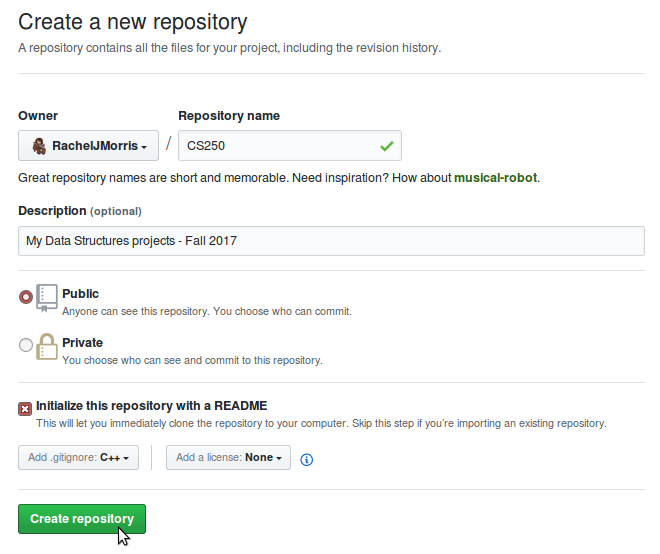
\includegraphics[width=14cm]{images/github-newrepo.png}
                \end{figure}

                Once you've set it up, click \textbf{Create repository}.
                It will then take you to the repository page. Leave this
                open, we will return to it later.

            \newpage
            
        \subsection{Installing Git}

            Next, you will need to set up Git on your machine. The
            offical Git website is at: https://git-scm.com/

        \paragraph{Lab computer:}
            If you're working on a lab computer, they should already have Git installed.

        \paragraph{Windows:}
            Go to the Downloads page and select the Windows download.
            Download either the 32-bit or 64-bit depending on
            your computer.

        \paragraph{Linux:}
            If you're using a Debian-based Linux distro, you can install it
            via the package manager or command line.

            ~\\
            Just search for ``git'' in the package manager...

                \begin{figure}[h]
                    \centering
                    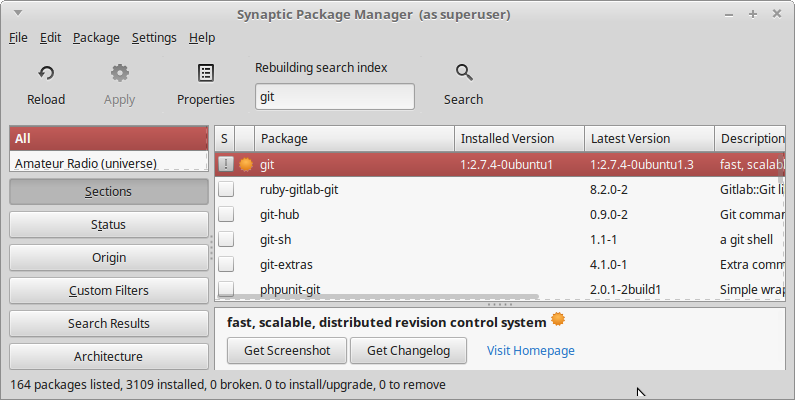
\includegraphics[width=14cm]{images/git-synaptic.png}
                \end{figure}

            ~\\
            Or open the terminal and use... \\
            \texttt{sudo apt-get install git}

                \begin{figure}[h]
                    \centering
                    
\includegraphics[width=14cm]{images/git-commandline-install.png}
                \end{figure}
            
        \paragraph{Mac:}

            I don't have a Mac computer I can test this out on. If there's
            a package manager for Mac, try to install it from there first.
            Otherwise, download the Mac package off the Git website.

        \subsection{Cloning the repository}

            Next, locate a place on your computer where you will want
            your CS 250 repository folder to be located.
            Right-click here to open up \textbf{Git bash} (Windows/Mac?)
            or the terminal (Linux). We will be using Git from the command
            line, but there are also GUI interfaces for it.

            Back on your profile page on the GitHub website, click on
            \textbf{Clone or download}. Make sure HTTPS is selected (you
            can set up SSH later if you want), and copy the URL given.

                \begin{figure}[h]
                    \centering
                    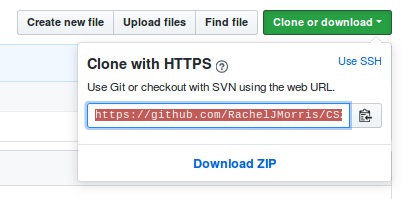
\includegraphics[height=5cm]{images/git-cloneurl.png}
                \end{figure}

            Back in the terminal, type ``git clone'' and then paste
            in the URL.

                \begin{figure}[h]
                    \centering
                    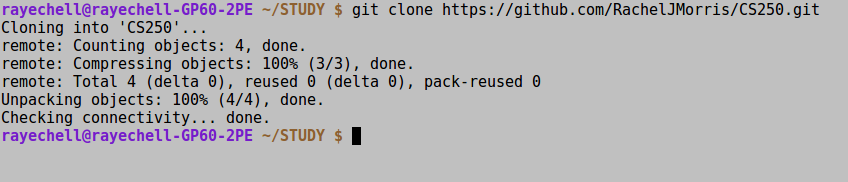
\includegraphics[width=14cm]{images/git-cl-clone.png}
                \end{figure}

            This will create a folder in the directory you chose.

                \begin{figure}[h]
                    \centering
                    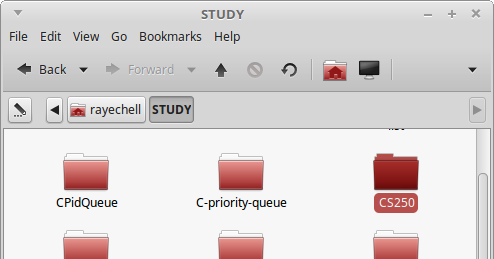
\includegraphics[width=8cm]{images/git-directory.png}
                \end{figure}

            Now you can do all your work in this folder, and any changes
            that you commit can be pushed to the server.

    \newpage

    \section{Moving your files over}
    
        Now you will move over your project files from class this semester
        into this repository folder. This should include your lab and project
        files. For example:

        \renewcommand*\DTstylecomment{\rmfamily\color{green}\textsc}

        \begin{framed}
        \dirtree{%
        .1 CS 250/.
        .2 Labs/.
        .3 Lab 01 - STL/.
        .3 Lab 02 - Exception Handling/.
        .3 Lab 03 - Static Array Wrapper/.
        .3 Lab 04 - Testing/.
        .3 Lab 05 - Dynamic Array Wrapper/.
        .3 Lab 08 - Templates/.
        .3 Lab 09 - Polymorphism/.
        .3 Lab 11 - Priority Queue/.
        .3 Lab 12 - Dictionary/.
        .3 Lab 14 - Recursion/.
        .2 Projects/.
        .3 Project 1 - Linked List/.
        .3 Project 2 - Stacks and Queues/.
        .3 Project 3 - Binary Search Trees/.
        }
        \end{framed}

    \section{Add, Commit, Pull, Push}

        \subsection{Add files}

        Now, navigate to the base folder of the repository (The CS250 folder)
        and open Git bash or the terminal.

        There are several ways you can add files...

        \begin{figure}[h]
            \centering
            
\includegraphics[width=14cm]{images/git-add.png}
        \end{figure}

        \begin{itemize}
            \item   \texttt{git add FILENAME} \\ Add a single file
            \item   \texttt{git add *.cpp} \\ Add everything that is a ``.cpp'' file in all subdirectories.
            \item   \texttt{git Labs/*} \\ Add ALL changes in the Labs folder and subdirectories in Labs/
            \item   \texttt{git add .} \\ Add ALL changes in all subdirectories.
        \end{itemize}

        Generally, you shouldn't add any .exe files, or other files that are
        generated each time the project is built. There's no reason to keep these
        in source control because they're auto-generated.

        You can store your project files if you'd like, though Visual Studio
        project files tend to be big.

        If you want to stick to the basics, just commit any .cpp, .hpp, .txt,
        and .csv files with the command I used in the screenshot:

        \begin{center}
            \texttt{git add *.cpp *.hpp *.txt *.csv}
        \end{center}

        The * is a wild-card, meaning ``anything can go here''. Since each
        item is *.EXTENSION, it will be any file as long as it matches the
        ending extension.

        If you want to double-check what you're adding, type:

        \begin{center}
            \texttt{git status}
        \end{center}

        and it will give you a list of files waiting to be committed.

        \begin{figure}[h]
            \centering
            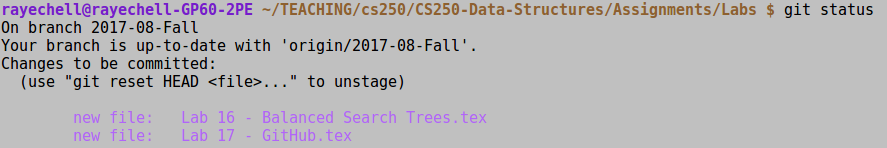
\includegraphics[width=14cm]{images/git-status.png}
            \caption{The CS 250 lab specs waiting to be committed. So meta.}
        \end{figure}

        \subsection{Commit files}

        Next, you will need to commit the changes. Each time you update
        files, you will need to \texttt{add} them, and then make a new
        \texttt{commit}. A commit can have multiple adds.

        To commit your changes with a message, use:

        \begin{center}
            \texttt{git commit -m "Adding my CS 250 files"}
        \end{center}

        It will display a list of the items being added. Since you're
        adding everything at once this time, it might be a huge list!

    \newpage

        \subsection{Pull and Push files}

        Making commits only stores the changes locally on your machine.
        When you're ready to push your changes up to the server, you will
        use the \texttt{push} command.

        However, if you're working across multiple computers, or with other people,
        it would be good to practice pulling prior to every push.
        \texttt{pull} pulls all the files from the server and performs
        a merge on anything that's changed.

        \begin{center}
            \texttt{git pull}
        \end{center}

        Right now, pull will just say that everything is up-to-date
        because nobody else is working in your repository. After the
        pull, make sure to push your changes.

        \begin{center}
            \texttt{git push}
        \end{center}

        It will have some messages about setting up defaults. There are
        a lot of extra features of Git that you can study up on later,
        but these are just the basics!

        It will push all updates to the server and display the status:
        
        \begin{figure}[h]
            \centering
            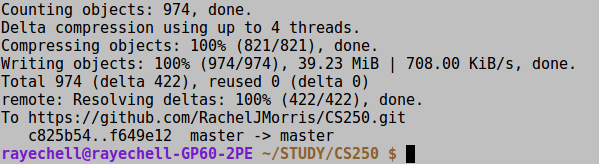
\includegraphics[width=14cm]{images/git-pushed.png}
            \caption{A successful push}
        \end{figure}
        
    \newpage

    \section{Viewing on the web interface}

        Once your changes have been pushed, you can now view them on the
        web interface:

        \begin{center}
        \texttt{https://github.com/YOUR-NAME/REPOSITORY-NAME}
        \end{center}
        
        \begin{figure}[h]
            \centering
            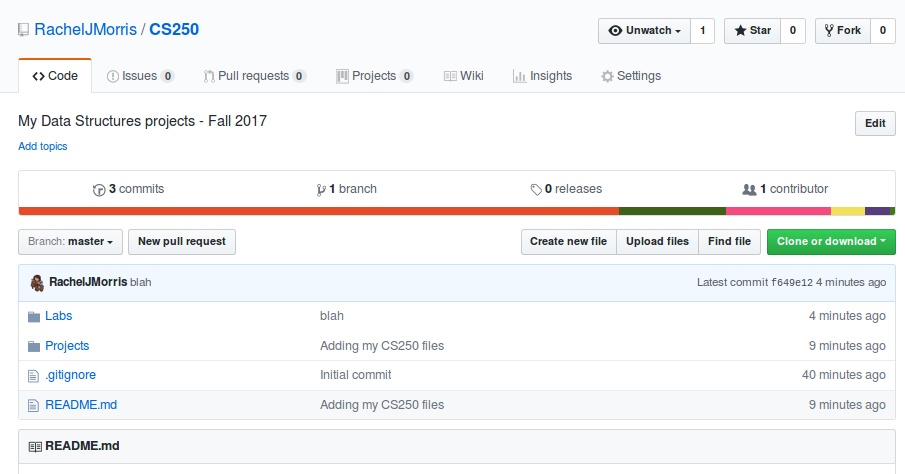
\includegraphics[width=14cm]{images/github-webrepo.png}
            \caption{Repository on the web}
        \end{figure}

        \subsection{Commit history (FYI)}

        Click on the \textbf{commits} link from the web interface.

        \begin{figure}[h]
            \centering
            
\includegraphics[width=5cm]{images/github-commits.png}
            \caption{Repository on the web}
        \end{figure}
        
        It will bring up a list of all the commits done in this repository.

        \begin{figure}[h]
            \centering
            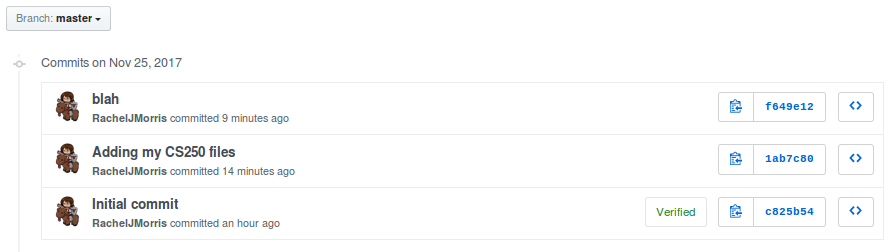
\includegraphics[width=14cm]{images/github-commits2.png}
            \caption{Viewing all commits}
        \end{figure}

        You can click on a commit message to view all the changes for all
        the files.

        \begin{figure}[h]
            \centering
            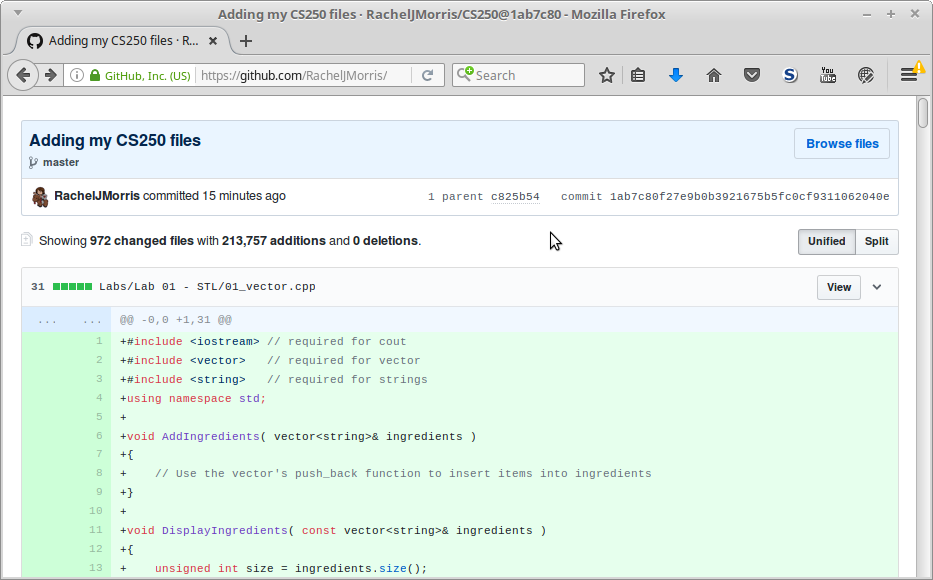
\includegraphics[width=14cm]{images/github-commits3.png}
            \caption{Viewing one commit}
        \end{figure}

    \newpage

    \subsection{Wiki (FYI)}

        If you click on the \textbf{Wiki} tab, you can create a little
        Wiki for your repository. This could be useful for projects
        where you want to add documentation for users to read.

        \begin{figure}[h]
            \centering
            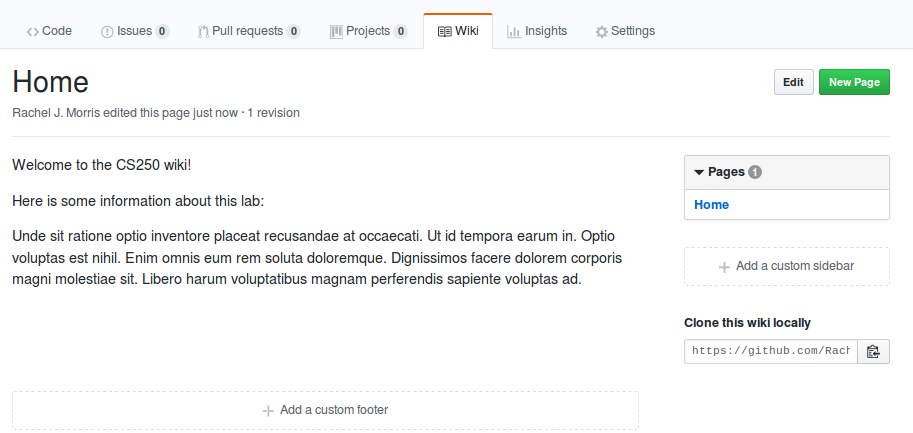
\includegraphics[width=14cm]{images/github-wiki.png}
        \end{figure}

    \hrulefill

    \subsection{Issues (FYI)}

        You can also use GitHub's \textbf{Issues} interface to keep
        up a ``to-do'' list of items to add, bugs to fix, etc.

        \begin{figure}[h]
            \centering
            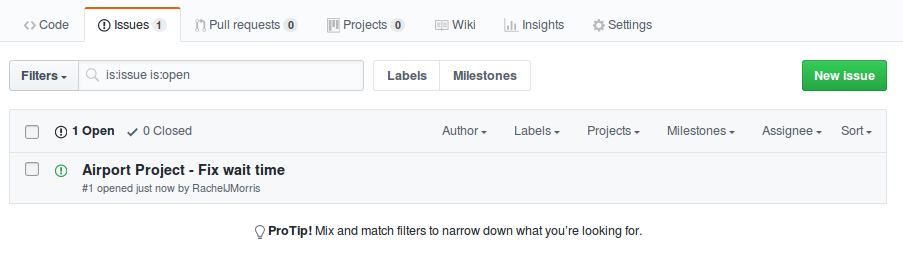
\includegraphics[width=14cm]{images/github-issues.png}
        \end{figure}

    \newpage

    \subsection{Pages (FYI)}

        You can also set up a simple webpage for each of your repositories,
        or even for your entire profile, with GitHub's Pages features.

        Go to \textbf{Settings} and scroll down to \textbf{GitHub Pages}.
        You can generate a page by selecting \textbf{Choose a theme}.

        \begin{figure}[h]
            \centering
            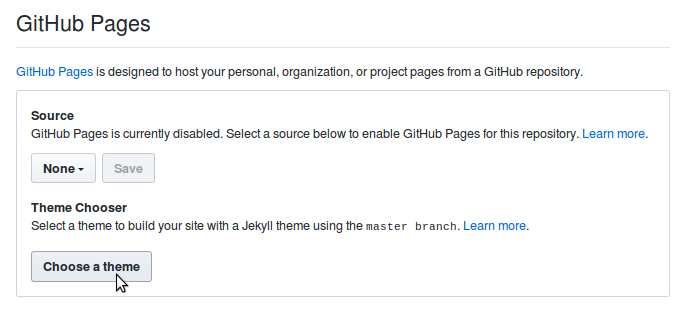
\includegraphics[width=14cm]{images/github-pages.png}
        \end{figure}

        After the page has been generated, you can go to \\
            \texttt{https://YOUR-NAME.github.io/YOUR-REPOSITORY/}
        to view it.

        \begin{figure}[h]
            \centering
            
\includegraphics[width=8cm]{images/github-pages3.png}
        \end{figure}

        GitHub has tutorials on their website for how to work with Pages
        if you're interested.

        You can create a profile-based page as well (rather than just a
        Page for a repository), which is good for hosting a portfolio page on.

        

\end{document}









